\documentclass[10pt,a5paper,twoside]{book}
\usepackage[utf8]{inputenc}
\usepackage[czech]{babel}
\usepackage[T1]{fontenc}
\usepackage{amsmath}
\usepackage{amsfonts}
\usepackage{amssymb}
\usepackage{hyperref}
\usepackage[dvips]{graphicx}
\usepackage[top=2cm, left=1.5cm, bottom=1.5cm, includefoot]{geometry}
\usepackage{eso-pic}
\usepackage{pdfpages}
\usepackage{textpos}
\usepackage{titlesec}
\usepackage{verbatim}
\fontencoding{T1}
\fontfamily{cmss}
\fontseries{m}
\fontshape{n}
\setlength{\belowcaptionskip}{-15pt} % mezera za popiskem obrázku
\usepackage{xcolor}
\usepackage{pdfpages}
\titleformat{\section}
{\color{blue}\normalfont\Large\bfseries}
{\color{blue}\thesection}{1.2em}{}

\newcommand{\autor}[1]{
	\begin{flushright}
	\textit{#1}
	\end{flushright}
}

\newcommand{\nadpis}[2]{
\section*{#1}
	\begin{flushright}
	\textit{#2}
	\end{flushright}
}

\newcommand{\podpis}[1]{
	\begin{flushright}
	\textit{#1}
	\end{flushright}
}

\begin{document} 



\section*{K obrázku na titulní straně}
popis titulniho obrazku ...
\vfill
\section*{JihoČAS}
Vydává: Jihočeská pobočka České astronomické společnosti.\\
Redakce a adresa pro zasílání příspěvků: Martin Kákona, U Jatek 19/III, 392 01 Soběslav, e-mail: \href{mailto:martin.kakona@astro.cz}{martin.kakona@astro.cz}.\\
Sazba: Roman Dvořák, e-mail: \href{mailto:roman-dvorak@email.cz}{roman-dvorak@email.cz}.\\
Vytisknuto s laskavým přispěním Jednoty České Budějovice.\newpage

\nadpis{Jak tuto šablonu používat?}{Roman Dvořák}






\begin{figure}[htbp]
	\begin{center}
		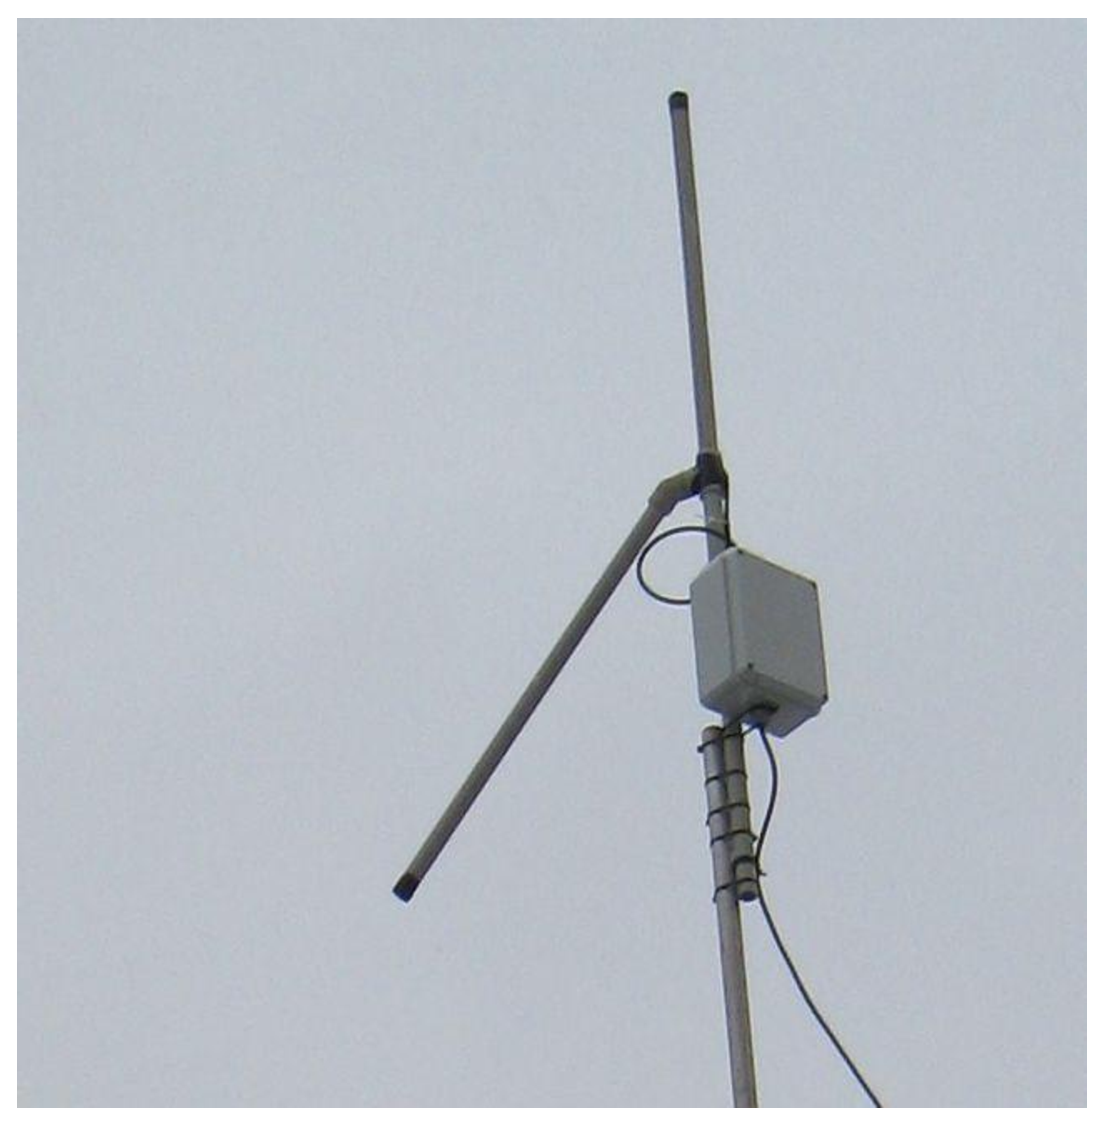
\includegraphics[width=7cm]{graves/graves_soubory/image005.eps}
	  	\caption{Možná konstrukce přijímací antény.}
	  	\label{fig:}
	\end{center}
\end{figure}

\end{document}
 
 
%	\begin{itemize}
%	\item 
%	\end{itemize}
